\documentclass[usenames,dvipsnames]{beamer}




% For more themes, color themes and font themes, see:
% http://deic.uab.es/~iblanes/beamer_gallery/index_by_theme.html
%
\mode<presentation>
{
  \usetheme{Madrid}       % or try default, Darmstadt, Warsaw, ...
  \usecolortheme{seagull} % or try albatross, beaver, crane, ...
  \usefonttheme{default}    % or try default, structurebold, ...
  \setbeamertemplate{navigation symbols}{}
  \setbeamertemplate{caption}[numbered]
} 



\newcommand\pro{\item[$+$]}
\newcommand\con{\item[$-$]}

\usepackage{xcolor}
\usepackage{hyperref}
\usepackage{amsmath}
\usepackage[english]{babel}
\usepackage[utf8x]{inputenc}

\usepackage{listings}

\lstset{
  commentstyle=\color{ForestGreen},
  backgroundcolor=\color{white},   % choose the background color; you must add \usepackage{color} or \usepackage{xcolor}; should come as last argument
  basicstyle=\ttfamily\scriptsize,        % the size of the fonts that are used for the code
  breakatwhitespace=false,         % sets if automatic breaks should only happen at whitespace
  breaklines=true,                 % sets automatic line breaking
  captionpos=b,                    % sets the caption-position to bottom
  deletekeywords={...},            % if you want to delete keywords from the given language
  escapeinside={\%*}{*)},          % if you want to add LaTeX within your code
  extendedchars=true,              % lets you use non-ASCII characters; for 8-bits encodings only, does not work with UTF-8
  frame=single,	                   % adds a frame around the code
  keepspaces=true,                 % keeps spaces in text, useful for keeping indentation of code (possibly needs columns=flexible)
  keywordstyle=\color{blue},       % keyword style
  language=java,                 % the language of the code
  morekeywords={contract, uint, constructor, function, pragma, solidity, *},            % if you want to add more keywords to the set
  numbers=left,                    % where to put the line-numbers; possible values are (none, left, right)
  numbersep=5pt,                   % how far the line-numbers are from the code
  numberstyle=\tiny\color{gray}, % the style that is used for the line-numbers
  rulecolor=\color{black},         % if not set, the frame-color may be changed on line-breaks within not-black text (e.g. comments (green here))
  showspaces=false,                % show spaces everywhere adding particular underscores; it overrides 'showstringspaces'
  showstringspaces=false,          % underline spaces within strings only
  showtabs=false,                  % show tabs within strings adding particular underscores
  stepnumber=2,                    % the step between two line-numbers. If it's 1, each line will be numbered
  stringstyle=\color{orange},     % string literal style
  tabsize=2,	                   % sets default tabsize to 2 spaces
  title=\lstname                   % show the filename of files included with \lstinputlisting; also try caption instead of title
}

\setlength\itemsep{2em}

% adapted from https://tex.stackexchange.com/questions/89574/language-option-supported-in-listings
\lstdefinelanguage{Solidity}{
	keywords={typeof, new, true, false, catch, function, return, null, catch, 
		switch, var, if, in, while, do, else, case, break, uint8, public, 
		private, internal, external, view, 	returns, emit, require, pragma,
		solidity, contract, address, event,	modifier, constructor},
	keywordstyle=\color{blue}\bfseries,
	ndkeywords={class, export, boolean, throw, implements, import, this},
	ndkeywordstyle=\color{darkgray}\bfseries,
	identifierstyle=\color{black},
	sensitive=false,
	comment=[l]{//},
	morecomment=[s]{/*}{*/},
	commentstyle=\color{purple}\ttfamily,
	stringstyle=\color{orange}\ttfamily,
	morestring=[b]',
	morestring=[b]"
}

\usepackage{tikz}
\usetikzlibrary{automata}
\usetikzlibrary{positioning}


% Here's where the presentation starts, with the info for the title slide
\title{Ethereum}
\subtitle{Introduction and overview of existing verification procedures}
\author{Mirko Bez}
\institute{Università di Padova}
\date{\today}

\begin{document}

\begin{frame}
  \titlepage
\end{frame}


%% GOALS
\begin{frame}{Blockchain Technology - Goals}
    \begin{itemize}

        \item Provide a \textbf{total order of the transactions} in a 
        distributed ledger without relying on a trusted third party (e.g. a 
        Bank)
        
        \item Avoid double spending problem (?)
        
        \item Avoid transaction repudiation (Signature)
        
        \item Immutability
        
    \end{itemize}
\end{frame}

\begin{frame}{Applications}
    
    \begin{block}{Applications}
        \begin{itemize}
            \item Financial Applications
            \item Auctions
            \item Elections
            \item Public sector (e.g. bureaucracy)
            \item Supply Chain
            \item etc.
        \end{itemize}
    \end{block}

    \begin{block}{Typologies}
        Permissionless vs Permissioned
    \end{block}
    
    
\end{frame}



%% Bitcoin
\begin{frame}{Bitcoin~\cite{nakamoto2008bitcoin}}
    \begin{itemize}
        \item P2P payment system
        \item Effectively, a \textbf{State Transition System} ($\sigma \xrightarrow{T} \sigma'$)
        \item The State is the balance of the
        addresses (UTXO list)
            \begin{itemize}
            \item Addresses are public keys, the users keep the private key secret
            \end{itemize}
        % \item A transaction may contain more than one input and more than one output addresses
        \item The transactions are collected in blocks
        $$
        \sigma_{0} \xrightarrow{B} \sigma_n \equiv 
        \sigma_{0} \xrightarrow{T_1} \sigma_1 \xrightarrow{T_2} \cdots
        \sigma_{n-1} \xrightarrow{T_n} \sigma_{n}
        $$
        \item The blocks are chained, thus forming a Blockchain 
    \end{itemize}
\end{frame}

\begin{frame}{Bitcoin~\cite{nakamoto2008bitcoin}}
\begin{itemize}
    \item Nodes execute client program (C++, Go, \dots)
    \item Structured overlay network
    \item Transactions and new blocks spread using \textbf{gossip protocols}
    \item Each peer maintains \emph{locally}:
    \begin{itemize} 
        \item a copy of the \emph{entire} \textbf{Blockchain}
        \item a copy of the \emph{entire} \textbf{State}
    \end{itemize}
    
    \item Each peers should:
    \begin{itemize}
        \item Accept only valid blocks with valid transactions
        %~ \item Check the validity that each transaction of the block is valid
        \item Update \textbf{its own} State according to the transactions
        %\item Each peer is aware of the whole transaction history  $\implies$ 
        %avoid double spending problem
    \end{itemize}
\end{itemize}

\end{frame}



\begin{frame}{Bitcoin~\cite{nakamoto2008bitcoin}}
\begin{block}{Script}
    \begin{itemize}
    \item Stack-based \textbf{Turing-incomplete} Language
    % \item Expresses conditions that should be full-filled to spend money
    \item UTXO have locking script
    \item Transaction input have unlocking script
    %\item Unlocking script solves a locking script, part of every tx input
    %it specifies the conditions that must be met to spend the output in the future:
    %\item Unlocking script solves a locking script, part of every tx input
    \item Validator/Miner executes locking and unlocking script together
    \item Stateless
    \end{itemize}
    \end{block}
    
    \begin{center}
    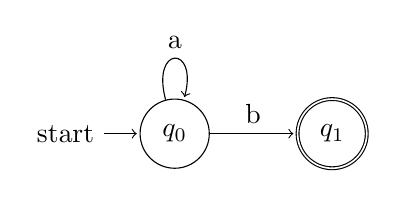
\begin{tikzpicture}[shorten >=1pt,node distance=2cm,on grid,auto] 
    \node[state,initial] (q_0)   {$q_0$}; 
    \node[state,accepting] (q_1) [right=of q_0]{$q_1$}; 
        \path[->] 
        (q_0) edge [loop above] node {a} ()
              edge node {b} (q_1);
    \end{tikzpicture}
    \end{center}
\end{frame}


\begin{frame}{Bitcoin~\cite{nakamoto2008bitcoin} - Consensus}

\begin{block}{Consensus}
  \begin{itemize}
  \item Avoid rewriting of history (Sybil Att.) Proof-of-Work (PoW)
  %~ \begin{itemize}
  %~ \item Find a nonce such that the hash of the block contains a certain
  %~ amount of leading zeros
  %~ \end{itemize}
  \item \textbf{Selection Rule}: Longest chain rule
  \end{itemize}
\end{block}

\begin{block}{Miners}
\begin{itemize}
\item Miners form the blocks
\item They decide which transactions are included and their \textbf{order}
\item They should mine valid blocks (e.g. balances always $\geq 0$)
\item They receive a reward
\end{itemize}
\end{block}

\end{frame}


\begin{frame}{Ethereum - Overview~\cite{bib:yellow}}
\begin{itemize}
\item Generalization of Bitcoin
\item Support execution of \emph{quasi-}Turing Complete smart contracts
\begin{itemize}
\item Avoid abuse of network resources
\item Each operation/opcode is associated with
an amount of gas % $\implies$ termination guaranteed
\item Gas price is determined per-transaction
\end{itemize}
\end{itemize}
\end{frame}

%% Ethereum Intro
\begin{frame}{Ethereum - World State~\cite{bib:yellow}}
	 Save the (World/Global) State ($\sigma$) explicitly
     \begin{itemize}
     \item Partial function from Addresses to Account States
     \item Externally owned account vs Contract Account
    \end{itemize}	
	 
    \begin{figure}
        \begin{center}
            \includegraphics[width=0.91\textwidth]{./img/world-state}
        \end{center}
    \end{figure}
\end{frame}

\begin{frame}{Ethereum - Tx Execution~\cite{bib:yellow}}
%\begin{itemize}
%\item Transactions alter the state
%    \begin{itemize}
%    	\item Message Call
%        \item Contract Creation
%    \end{itemize}
%\end{itemize}
\begin{center}
\includegraphics[height=0.95\textheight]{./img/transaction-execution}
\end{center}
\end{frame}


\begin{frame}{Execution Model - EVM~\cite{bib:yellow}}
\begin{center}
\includegraphics[width=0.8\textwidth]{./img/evm-overview}
\end{center}
\end{frame}

% EVM specifica nello yellow paper + molteplici formalizzazioni
% in letteratura


\begin{frame}{Future directions}
\begin{itemize}
\item Proof-of-Stake
\item Sharding
\end{itemize}
\end{frame}


\begin{frame}[fragile]{Solidity}
    \begin{itemize}
        \item \emph{Contract-oriented}
        \item Statically typed
        \item Primitives to access environment data %\item
        \item Contract interfaces, inheritance, abstract contracts, libraries
        \item Support for inline assembly
        \item Expressivity leads to potential vulnerabilities
        \item First formalization attempts with \href{https://github.com/kframework/solidity-semantics}{$\mathbb{K}$-Framework}
    \end{itemize}
\end{frame}

\begin{frame}[fragile]{Solidity - Functions}
        \begin{itemize}
        \item Function Selector \\
        \lstinline!bytes4(keccak256("foo(uint8,uint16)"))!
        \item Fallback Function \\
        \lstinline!function () public { }!
        \item \texttt{external/internal/private/public}
        \item \texttt{view/pure/payable}
        \item Modifiers
        \end{itemize}
\end{frame}


\begin{frame}[fragile]{Solidity Example}
\begin{lstlisting}[frame=single, language=Solidity]
pragma solidity ^0.4.24;
contract Example {
    uint8 public x; 
    address private owner;
    
    constructor() public { x = 0; owner = msg.sender; }
    
    event XHasChanged(uint8 oldValue, uint8 newValue);
    
    modifier onlyOwner() {
        require(msg.sender == owner);
        _; //Placeholder for the body of the function
    }
    
    function modifyX(uint8 newValue) 
    public onlyOwner returns (uint8 oldValue) {
        oldValue = x;
        x = newValue;
        emit XHasChanged(oldValue, newValue);
    }
}

\end{lstlisting}

\end{frame}


\begin{frame}{Vyper~\cite{bib:vyper-docs}}

  \begin{itemize}
  	\item \textbf{Aim:} Write secure, human-readable  contracts:
  	\begin{itemize}
  		\item It gives up: modifiers, inheritance, inline assembly, function overloading, recursive calls, Infinite-length loops
  	\end{itemize}
    \item predictable gas consumption
    \item Resembles python
  	\item \href{https://github.com/kframework/vyper-semantics/}{Formalization in $\mathbb{K}$-Framework}
  \end{itemize}

\end{frame}


\begin{frame}{EVM Alternative Languages}
\begin{block}{Bamboo~\cite{bamboo}}
\begin{itemize}
\item Polymorphic contracts: According to the stages, a contract changes its signature
\item Do not support loops
\end{itemize}
\end{block}

\begin{block}{Obsidian~\cite{obsidian}}
  \begin{itemize}
  \item State as first class citizen
  \item The methods that can be invoked on an object depend on the object’s current state.
  \end{itemize}
\end{block}
\end{frame}



\begin{frame}{Future directions}
    \begin{itemize}
        \item Proof-of-Stake
        \item Sharding
    \end{itemize}
\end{frame}


\begin{frame}[allowframebreaks]
        \frametitle{References}
        \bibliographystyle{apalike}
        \bibliography{bibliography.bib}
\end{frame}

\end{document}

